\newpage
\section{Klassifikation}\label{kap:klassifikation}
In Kapitel \ref{kap:detektion} wurde beschrieben, wie die Positionen aller Kugeln mithilfe eines Bilds des Spielstands detektiert werden.
Um den Spielstand zu verstehen ist es relevant zu wissen, welche Kugel welche Farbe hat.
Im Snooker gibt es die Farben Weiss, Rot, Gelb, Pink, Grün, Blau, Braun und Schwarz.
Deshalb muss jede detektierte Kugel anhand eines Bildausschnitts in eine dieser Klassen eingeteilt werden.
Der Ablauf der Klassifikation der Snooker-Kugeln wird nachfolgend beschrieben.

Zunächst liegt zu jeder Kugel deren Position in Pixel- sowie Modell-Koordinaten vor und der Radius der Kugeln ist in Pixel bekannt\cite{project2:pixel_to_model_coordinates}.
Aufgrund dieser Informationen wird von jeder detektierten Kugel ein Bildausschnitt des RGB-Bildes rund um die Kugelposition definiert,
der für die Klassifikation verwendet werden kann.
Der Bildausschnitt ist quadratisch, wodurch in den Ecken des Bildes noch das Grün des Billardtisches ersichtlich ist.
% TODO: bilder dazu einfügen

Dieses Grün könnte die Klassifikation verfälschen, da damit mehr grüne Pixel auf dem Bild sind und eine Kugel eher als grün klassifiziert werden könnte.
Um dieses Problem zu umgehen wird der Pixelradius der Kugel mit einem Faktor von $0.5$ skaliert, um den Bildausschnitt zu verkleinern
und den grünen Tisch so zu entfernen.

Als Nächstes wird zur Rauschunterdrückung ein Gauss-Filter mit der Kernelgrösse von 5x5 auf den Bildausschnitt angewendet.
Anschliessend wird das RGB-Bild in den HSV-Farbraum\cite{wiki:hsv_color_space} konvertiert, um die Farbanalyse zu vereinfachen.
Aufgrund des HSV-Bildes wird pro Kanal (Hue, Saturation und Value) ein Histogramm berechnet und der häufigste Wert ermittelt.
Damit wurde die Information des Bildausschnitts auf drei Zahlen, eine pro HSV-Kanal, reduziert.
Diese drei Werte können als Position des Bildausschnitts im HSV-Raum interpretiert werden.

Pro Kugelfarbe kann definiert werden, in welche HSV-Bereiche diese Kugeln gehören. Bspw. gehören Rot, Pink, Braun eher in den roten
Bereich des Hue-Kanals. Blau, Gelb und Grün sind vom roten Bereich abgrenzbar.
Die weisse und schwarze Kugel sind am ehesten im Value-Kanal klassifizierbar.

Für eine genauere Unterscheidung wurden Bilder von verschiedenen Spielständen gemacht und anhand dieser die genauen Parameter
für die Klassifikation gefunden. In diesen Trainingsbildern ist eine Kugel jeder Klasse an unterschiedlichen Stellen platziert worden,
um die ungleichmässige Ausleuchtung des Billardtischs zu berücksichtigen.
In Abbildung \ref{fig:classification_trainingdata_examples} sind zwei Trainingsbilder pro Klasse aufgeführt.

\begin{figure}[h!]
    \centering
    \begin{subfigure}[b]{0.15\textwidth}
        \centering
        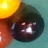
\includegraphics[width=1.0\linewidth]{../common/03_billiard_ai/resources/classification/BLACK_1.png}
        \caption{Schwarz 1}
        \label{fig:classification_black_ball_1}
    \end{subfigure}
    \hfill
    \begin{subfigure}[b]{0.15\textwidth}
        \centering
        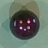
\includegraphics[width=1.0\linewidth]{../common/03_billiard_ai/resources/classification/BLACK_2.png}
        \caption{Schwarz 2}
        \label{fig:classification_black_ball_2}
    \end{subfigure}
    \hfill
    \begin{subfigure}[b]{0.15\textwidth}
        \centering
        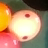
\includegraphics[width=1.0\linewidth]{../common/03_billiard_ai/resources/classification/WHITE_1.png}
        \caption{Weiss 1}
        \label{fig:classification_white_ball_1}
    \end{subfigure}
    \hfill
    \begin{subfigure}[b]{0.15\textwidth}
        \centering
        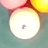
\includegraphics[width=1.0\linewidth]{../common/03_billiard_ai/resources/classification/WHITE_2.png}
        \caption{Weiss 2}
        \label{fig:classification_white_ball_2}
    \end{subfigure}
    \hfill
    \begin{subfigure}[b]{0.15\textwidth}
        \centering
        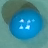
\includegraphics[width=1.0\linewidth]{../common/03_billiard_ai/resources/classification/BLUE_1.png}
        \caption{Blau 1}
        \label{fig:classification_blue_ball_1}
    \end{subfigure}
    \hfill
    \begin{subfigure}[b]{0.15\textwidth}
        \centering
        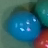
\includegraphics[width=1.0\linewidth]{../common/03_billiard_ai/resources/classification/BLUE_2.png}
        \caption{Blau 2}
        \label{fig:classification_blue_ball_2}
    \end{subfigure}
    \hfill
    \begin{subfigure}[b]{0.15\textwidth}
        \centering
        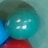
\includegraphics[width=1.0\linewidth]{../common/03_billiard_ai/resources/classification/GREEN_1.png}
        \caption{Grün 1}
        \label{fig:classification_green_ball_1}
    \end{subfigure}
    \hfill
    \begin{subfigure}[b]{0.15\textwidth}
        \centering
        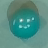
\includegraphics[width=1.0\linewidth]{../common/03_billiard_ai/resources/classification/GREEN_2.png}
        \caption{Grün 2}
        \label{fig:classification_green_ball_2}
    \end{subfigure}
    \hfill
    \begin{subfigure}[b]{0.15\textwidth}
        \centering
        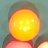
\includegraphics[width=1.0\linewidth]{../common/03_billiard_ai/resources/classification/YELLOW_1.png}
        \caption{Gelb 1}
        \label{fig:classification_yellow_ball_1}
    \end{subfigure}
    \hfill
    \begin{subfigure}[b]{0.15\textwidth}
        \centering
        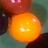
\includegraphics[width=1.0\linewidth]{../common/03_billiard_ai/resources/classification/YELLOW_2.png}
        \caption{Gelb 2}
        \label{fig:classification_yellow_ball_2}
    \end{subfigure}
    \hfill
    \begin{subfigure}[b]{0.15\textwidth}
        \centering
        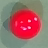
\includegraphics[width=1.0\linewidth]{../common/03_billiard_ai/resources/classification/RED_1.png}
        \caption{Rot 1}
        \label{fig:classification_red_ball_1}
    \end{subfigure}
    \hfill
    \begin{subfigure}[b]{0.15\textwidth}
        \centering
        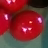
\includegraphics[width=1.0\linewidth]{../common/03_billiard_ai/resources/classification/RED_2.png}
        \caption{Rot 2}
        \label{fig:classification_red_ball_2}
    \end{subfigure}
    \hfill
    \begin{subfigure}[b]{0.15\textwidth}
        \centering
        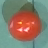
\includegraphics[width=1.0\linewidth]{../common/03_billiard_ai/resources/classification/BROWN_1.png}
        \caption{Braun 1}
        \label{fig:classification_brown_ball_1}
    \end{subfigure}
    \hfill
    \begin{subfigure}[b]{0.15\textwidth}
        \centering
        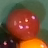
\includegraphics[width=1.0\linewidth]{../common/03_billiard_ai/resources/classification/BROWN_2.png}
        \caption{Braun 2}
        \label{fig:classification_brown_ball_2}
    \end{subfigure}
    \hfill
    \begin{subfigure}[b]{0.15\textwidth}
        \centering
        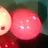
\includegraphics[width=1.0\linewidth]{../common/03_billiard_ai/resources/classification/PINK_1.png}
        \caption{Pink 1}
        \label{fig:classification_pink_ball_1}
    \end{subfigure}
    \hfill
    \begin{subfigure}[b]{0.15\textwidth}
        \raggedright
        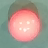
\includegraphics[width=1.0\linewidth]{../common/03_billiard_ai/resources/classification/PINK_2.png}
        \caption{Pink 2}
        \label{fig:classification_pink_ball_2}
    \end{subfigure}
    \caption{Auswahl aus den Trainingsbilder}
    \label{fig:classification_trainingdata_examples}
\end{figure}

Das Resultat der Analyse dieser Daten sind Wertebereiche für die HSV-Kanäle pro Klasse, wodurch eine grobe Klassifikation,
ermöglicht wird. Diese Wertebereiche bieten keine eindeutige Klassifikation, sondern werden verwendet, um die potentiellen
Klassen einer Kugel zu finden.
So kann es sein, dass eine blaue Kugel aufgrund ihres Hue-Kanals klar als Blau erkannt wird.
Es kann aber auch sein, dass eine braune Kugel sowohl Rot, Pink und Braun als potentielle Klassen erhält.

Es muss demnach noch eine genauere Unterscheidung gemacht werden, sobald die potentiellen Klassen bekannt sind.
Anhand der Trainingsbildern wurden die Durchschnittswerte der häufigsten Werte der HSV-Kanäle pro Klasse berechnet.
Diese Durchschnittswerte bilden die Cluster-Zentren jeder Klasse und können für die Klassifikation verwendet werden.
Dazu wird die Distanz der HSV-Position des zu klassifizierenden Bildausschnitts zu jedem Cluster-Zentrum bestimmt.
Der Cluster mit der kleinsten Distanz gibt dem Bildausschnitt seine Klasse.

Sofern ein Bildausschnitt mehrere potentielle Klassen in der Prüfung durch Wertebereiche erhalten hat, wird die Distanz
zwischen dessen HSV-Position und dem Cluster-Zentrum jeder der potentiellen Klassen verglichen.
Die Klasse mit der kleinsten Distanz zur HSV-Position des Bildausschnitts wird angenommen.
Demnach ist diese Klassifikation in der Idee ein \emph{k-nearest neighbors} Algorithmus\cite{wiki:k_nearest_neighbors},
wobei keine Trainingsdatensätze als Nachbaren verwendet werden, sondern die bereits gefundenen Cluster-Zentren.

Sofern ein Bildauschnitt keine potentiellen Klassen erhalten hat, wird diesem die Klasse \emph{unbekannt} zugewiesen.

Mit der hier beschriebenen Klassifikation ist die Farbe jeder Kugel nach deren Detektion bekannt und es
sind alle Informationen für die weitere Verwendung in der Suche und Darstellung vorhanden.
